\documentclass{article}
\usepackage{cite}
\usepackage[utf8]{inputenc}
\newcommand\independent{\protect\mathpalette{\protect\independenT}{\perp}}
\def\independenT#1#2{\mathrel{\rlap{$#1#2$}\mkern2mu{#1#2}}}
\title{Report for Comp Exam}
\author{Siyuan Zhao}
\date{April 2017}

\usepackage[linesnumbered,ruled]{algorithm2e}
\usepackage{amsmath, mathtools}
\usepackage{amsfonts}
\begin{document}

\maketitle
\section{Problem Setup}
\subsection{Randomized Controlled Trials}
In RCTs, participants are randomly assigned to conditions so treatment is assigned by randomization. As a consequence of
randomization, an unbiased estimate of the ATE can be directly
computed from the data. An unbiased estimate of the ATE is
$E[Y_i(1)-Y_i(0)]=E[Y(1)] - E[Y(0)]$.

\subsection{Observational Studies}
An observational study has the same intent as a randomized experiment:
to estimate a causal effect. However, an observational study differs
from a RCT in one design issue: the use of randomization to allocate
participants to treatment and control groups.

In observational studies, the treated subjects often differ
systematically from untreated subjects. In general, $E[Y(1)\mid t=1]
\neq E[Y(1)]$ holds. Thus, an unbiased estimate of the average
treatment effect cannot be obtained by directly comparing outcomes
between the the treated and the control groups.

\subsection{Strong Ignorability}
The treatment assignment is defined to be strongly ignorable
\cite{rosenbaum1983central} if the following two conditions hold: 1).
$(Y(1), Y(0)) \independent t\mid X$ and 2). $0 < \Pr (t=1 \mid X) <
1$. The first condition says that treatment assignment is independent
of the potential outcomes conditional on the observed features of subjects. The second condition says that every subject has a nonzero
probability to receive either treatment. The aforementioned first
condition is also referred to as the "no-hidden confounding variables"
assumption that all factors determining the outcome of each condition
are observed.

\section{Random Causal Forests}
\cite{wager2015estimation} proposed random causal forest (RCF) to
infer treatment effect. From the conceptual point of view, causal trees can be viewed as
nearest neighbor methods with an adaptive neighborhood metric. Assume
that there are $n$ observed independent samples $(X_i, Y_i,
W_i)_{i=1}^n$. The workflow of the RCF is that a causal tree is first
built by recursively splitting the feature space until all samples are
partitioned into a set of leaves $L$, each of which contains a few
training samples. Then, for a data point $x$, the predicted outcome $\hat{\mu}(x)$
is evaluated by identifying the leaf $L(x)$ containing $x$ and
calculating

$$\hat{\mu} = \frac{1}{\left | \left \{ i: X_i \in L(x) \right \}
  \right |} \sum_{\left \{ i: X_i \in L(x) \right \}} Y_i$$

Given a test point $x$, the closest points to $x$ are those fall in the same
leaf as it. The authors believe that the leaf is small enough that the
responses $Y_i$ are roughly identically distributed. Then the
treatment effect $\hat{\tau}$ for any $x \in L(x)$ is estimated as
following:

\begin{align} 
\hat{\tau}(x) & = \frac{1}{\left | \left \{ i: W_i=1, X_i \in L(x) \right \}
                \right |} \sum_{\left \{ i: W_i = 1, X_i \in L(x)
                \right \}} Y_i \nonumber \\
              & - \frac{1}{\left | \left \{ i: W_i=0, X_i \in L(x) \right \}
  \right |} \sum_{\left \{ i: W_i = 0, X_i \in L(x) \right \}} Y_i \label{eq:tree-treatment-effect}
\end{align}

RCF assumes that
there is overlapping in the data, i.e., for some $\epsilon > 0$ and
all $x \in \left [ 0, 1\right ]^d$,

$$\epsilon < \mathbb{P}\left [ W=1 \mid X=x \right ] < 1-\epsilon$$

This condition effectively guarantees that, for large enough $n$,
there will be enough treatment and control units near any test point
$x$ for local methods to work.

\subsection{Honest Trees and Forests}
The authors also define the Honest Trees and Forests in \cite{wager2015estimation}.
A tree is honest if, for each training example $i$, it only uses the
response $Y_i$ to estimate the within-leaf treatment effect $\tau$
using Equation~\ref{eq:tree-treatment-effect} or
to decide where to place the splits, but not
both. There are two causal forest algorithms proposed from
\cite{wager2015estimation} that satisfy this condition.

The first algorithm, which is called double-sample trees, achieves
honesty by dividing its training data into two halves
$\mathcal{I}$ and $\mathcal{J}$. Then, it uses the
$\mathcal{J}$-sample to place the splits, while holding out the
$\mathcal{I}$-sample to do within-leaf estimation. The details of the
algorithm is shown in Algorithm~\ref{algo:double-sample-trees}.

\LinesNumberedHidden
\begin{algorithm}[h]
  \SetKwInOut{Input}{Input}
  \Input{$n$ training examples of $(X_i, Y_i, W_i)$, where $X_i$ are
    features, $Y_i$ is the response, and $W_i$ is the treatment
    assignment. \\
    A minimum leaf size $k$.
  }

  \caption{Double-sample Causal Trees}~\label{algo:double-sample-trees}
  \ShowLn Draw a random subsample of size $s$ from $\{1, \ldots, n\}$ without
  replacement, and then divide it into two disjoint sets of size
  $|\mathcal{I}|=\left \lfloor s/2 \right \rfloor$ and
  $|\mathcal{J}|=\left \lceil s/2 \right \rceil$ \\
  \ShowLn Grow a tree via recursive partitioning. The splits are chosen using
  any data from the $\mathcal{J}$ sample and $X$- or $W$-observations
  from the $\mathcal{I}$ sample, but without using $Y$-observations
  from $\mathcal{I}$-sample. \\
  \ShowLn Estimate leaf-wise response using only the $\mathcal{I}$-sample
  observations. \\ [1\baselineskip]

The algorithm estimates $\hat{\tau}(x)$ using
Equation~\ref{eq:tree-treatment-effect} on the $\mathcal{I}$
sample. The splitting criteria is to maximize the variance of
$\hat{\tau}(X_i)$ for $i \in \mathcal{J}$. Each leaf of the tree must
contain $k$ or more $\mathcal{I}$-sample observations of each
treatment class.
\end{algorithm}
Another approach to build honest trees is inspired by the idea of
propensity score matching, which is called propensity trees. The idea
behind this approach is to train a classification tree to predict the
propensity score, which is the treatment assignments $W_i$, and ignore the outcome $Y_i$ when
placing splits. This method is useful in observational studies
since propensity score is aimed to reduce the selection bias by
equating groups based on these features. The details of the
algorithm is shown in Algorithm~\ref{algo:propensity-trees}.

\LinesNumberedHidden
\begin{algorithm}[h]
  \SetKwInOut{Input}{Input}
  \Input{$n$ training examples of $(X_i, Y_i, W_i)$, where $X_i$ are
    features, $Y_i$ is the response, and $W_i$ is the treatment
    assignment. \\
    A minimum leaf size $k$.
  }
  \ShowLn Draw a random subsample $\mathcal{I} \in {1, \ldots, n}$ of
  size $|\mathcal{I}| = s$ (no replacement). \\
  \ShowLn Train a classification tree using sample $\mathcal{I}$ where
  the outcome is the treatment assignment, i.e., on the $(X_i, W_i)$
  pairs with $i \in \mathcal{I}$. Each leaf of the tree must have $k$
  or more observations of each treatment class. \\
  \ShowLn Estimate $\tau(x)$ using
  Equation~\ref{eq:tree-treatment-effect} on the leaf containing $x$.
  \caption{Propensity Trees}~\label{algo:propensity-trees}
\end{algorithm}

\section{Counterfactual Inference}
The problem of causal inference is often framed in terms of
counterfactual problems such as "Would this particular student benefit
more from the video hint or the text hint when the student cannot
solve a problem?" In the binary intervention set, there are two possible interventions
$\mathcal{T} = \left \{  0, 1 \right \}$, where intervention 1 is
often referred as the "treated" and intervention 0 is the "control."
Given a sample of subjects and a treatment, each subject has a pair of
potential outcomes: $Y_0$ and $Y_1$, the outcomes under the
control and the treatment, respectively. Let $t$ be an indicator
variable denoting the treatment received ($t = 0$ for the control and
$t=1$ for the treatment). Only one outcome, which is called factual
outcome, $y_F(\mathbf{x}) =t\cdot Y_1(\mathbf{x}) +
(1-t) \cdot Y_0(\mathbf{x})$, is observed for the
subject $\mathbf{x}$, where
$\mathbf{x} \in \mathcal{X}$ are the
observed features for the subject. The unobserved outcomes are referred to as the
counterfactual outcome, denoted as $y_{CF}(\mathbf{x}) = (1-t)\cdot Y_1(\mathbf{x}) +
t \cdot Y_0(\mathbf{x})$. In other words, when a subject $\mathbf{x}$ is assigned to the
"control" ($t = 0$), $y_F(\mathbf{x})$ is equal to $Y_1(\mathbf{x})$, and $y_{CF}(\mathbf{x})$ is
equal to $Y_0(\mathbf{x})$. The other way around, $y_F(\mathbf{x})$ is equal to
$Y_0(\mathbf{x})$, and $y_{CF}(\mathbf{x})$ is equal to $Y_1(\mathbf{x})$. The estimated
individual treatment effect (ITE) is then calculated by
$\mathrm{ITE}(\mathbf{x})=Y_1(\mathbf{x}) - Y_0(\mathbf{x})$. The goal
of counterfactual inference is to predict the counterfactual outcome
given the observed data $D_n=\{(\mathbf{x}_i,t_i,y_F^i)_{i=1}^n\}$ from either RCTs or observational studies in
order to estimate the ITE.

We assume $n$ samples $\left \{ (x_i, t_i, y_F^i) \right \}_{i=1}^n$
form an empirical distribution $\hat{p}^F  = \left \{ (x_i, t_i)
\right \}_{i=1}^n$. We call this empirical distribution $\hat{p}^F
\sim p^F$ the empirical factual distribution. In order to calculate
ITE, we need to infer the counterfactual outcome which is dependent on
the empirical distribution $\hat{p}^{CF}  = \left \{ (x_i, 1-t_i)
\right \}_{i=1}^n$, which is called the empirical counterfactual distribution $\hat{p}^{CF}
\sim p^{CF}$. The $p^{F}$ and $p^{CF}$ may not be equal because the
distributions of the control and the treated populations may be
different. The inequality of two distributions may cause the
counterfactual inference over a different distribution than the one
observed from the experiment. In machine learning terms, this scenario
is usually referred to as domain adaptation, where the distribution of
features in test data are different than the distribution of features
in training data.

\cite{Johansson2016-dh} proposed Balancing Neural Networks (BNN) which
can be applied to solve the counterfactual inference problem. They
used a form of regularizer to enforce the similarity between the
distributions of representations learned for populations with
different interventions, for example, the representations for students
who received text hints versus those who received video hints.This
reduces the variance from fitting a model on one distribution and
applying it to another. Because of random assignment to the
interventions in RCTs, the distributions of the populations within
different interventions are highly likely to be identical. However, in
the observational study, we may end up with the situation where only
male students receive video hints and female students receive text
hints. Without enforcing the similarity between the distributions of
representations for male and female students, it is not safe to make a
prediction of the outcome if male students receive text hints.

The Counterfactual Regression (CFR) \cite{Shalit2016-qk} is built on the BNN. The important difference between these two models is that the CFR uses a more powerful distribution metric in the form of IPMs to learn a balancing representation.

\begin{figure}[h]
  \centering
  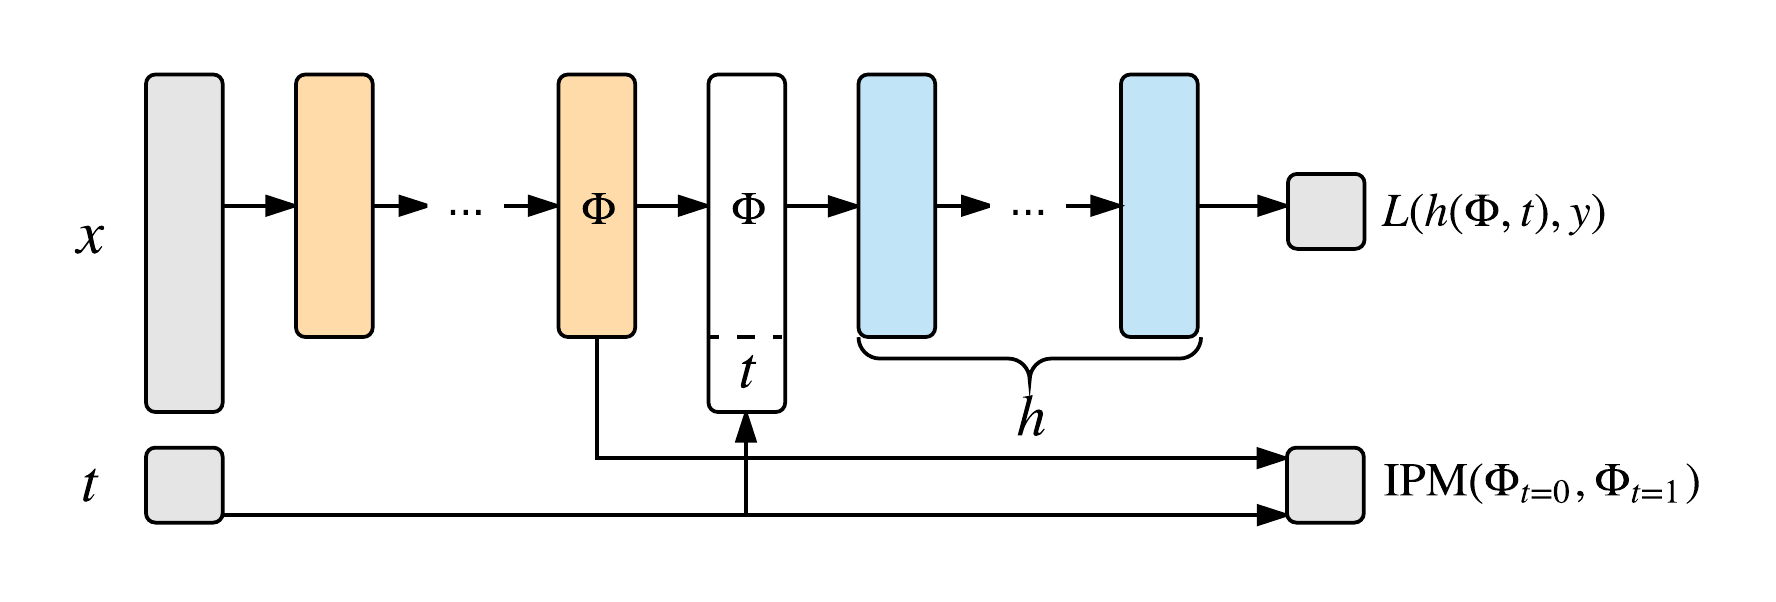
\includegraphics[width=0.95\columnwidth]{cfr.png}
  \caption{CFR for ITE estimation. $L$ is a loss function, IPM is an integral probability metric}.
  ~\label{fg:cfr-model}
\end{figure}

The structure of CFR is illustrated in Figure~\ref{fg:cfr-model}. To learn a representation of deep features $\Phi$, the CFR uses fully connected layers with ReLu activation function, where $Relu(z) = max(0, z)$. We need to generalize from factual distribution to counterfactual distribution in the feature representation $\Phi$ to obtain accurate estimation of counterfactual outcome. The common successful approaches for domain adaptation encourage similarity between the latent feature representations w.r.t the different distributions. This similarity is often enforced by minimizing a certain distance between the domain-specific hidden features. The distance between two distributions is usually referred to as the discrepancy distance, introduced by \cite{Mansour2009-fh}, which is a hypothesis class dependent distance measure tailored for domain adaptation. 

Integral Probability Metric (IPM) are used to measure the distance between two distributions $p_0 = p(x|t = 0)$, and $p_1 = p(x|t = 1)$, also known as the control and treated distributions. The IPM for $p_0$ and $p_1$ is defined as
$$\mathrm{IPM}_{\mathcal{F}}(p_0, p_1) := \sup_{f\in \mathcal{F}} \left |\int_S f dp_0 -\int_S f d p_1 \right |,$$

where $\mathcal{F}$ is a class of real-valued bounded measurable functions on $S$. 

The choice of functions is the crucial distinction between IPMs \cite{Sriperumbudur2009-pf}. Two specific IPMs are used in our experiments: the Maximum Mean Discrepancy (MMD), and the Wasserstein distance. $\mathrm{IPM}_{\mathcal{F}}$ is called MMD, when $\mathcal{F} = \left \{ f : \left \| f \right \| _\mathcal{H}\leq 1\right \}$, where $\mathcal{H}$ represents a reproducing kernel Hilbert space (RKHS) with $k$ as its reproducing kernel. In other words, the family of norm-1 reproducing kernel Hilbert space (RKHS) functions lead to the MMD. The family of 1-Lipschitz functions $\mathcal{F} = \left \{ f:\left \| f\right \|_L \leq 1 \right \}$, where $\left \| f\right \|_L$ is the Lipschitz semi-norm of a bounded continuous real-valued function $f$, make IPM the Wasserstein distance. Both the Wasserstein and MMD metrics have consistent estimators which can be efficiently computed in the finite sample case \cite{Sriperumbudur2012-sz}. The important property of IPM is that $$p_0 = p_1~\mathrm{iff}~ \mathrm{IPM}_{\mathcal{F}}(p_0, p_1) = 0.$$

The representation with reduction of the discrepancy between the control and the treated populations helps the model to focus on balancing features across two populations when inferring the counterfactual outcomes. For instance, if in an experiment, almost no male student ever received intervention A, inferring how male students would react to intervention A is highly prone to error and a more conservative use of the gender feature might be warranted.

After obtaining the representation for subject $\mathbf{x_i}$, CFR
concatenates the treatment assignment $t_i$ to the representation $\Phi(\mathbf{x}_i)$ and feeds $[\Phi(\mathbf{x}_i), t_i]$ to another two fully connected layers to generate the predicted outcome.
\section{Individualized Treatment Rules}
An individual treatment rule (ITR) $d: \mathcal{X} \rightarrow \mathcal{T}$ is a deterministic decision
rule from subject $\mathbf{x} \in \mathcal{X}$ into the intervention space $\mathcal{T}$. In experiments, we observe a triplet $(\mathbf{x}, t, y)$ from each
subject, where $\mathbf{x}=(x_1, x_2, \ldots, x_n)^T \in
\mathcal{X}$ denotes the participant's observed features, $t \in \mathcal{T}
= {-1,1}$ denotes the treatment assignment, and $y \in Y$ is the
observed outcome, also called the "reward" in the literature on
reinforcement learning. Note that $t=-1$ means that the subject is
assigned to the control and $t=1$ mean that the subject is assigned to
the treatment in the
context of ITR. Let $p(t|\mathbf{x})$ be the probability of assigning the subject
with features $\mathbf{x}$ to the intervention $t$. \cite{Qian2011-vz}
showed that the
value of $d$ satisfies
$$V(d) = E \left [ \frac{y}{p(t|x)}\mathbb{I}_{t=d(\mathbf{x})}\right
],$$
where $\mathbb{I}(\cdot)$ is an indicator function. The goal of the
ITR is to find an optimal ITR, $d^{*}$, which is a rule that has the maximal value such
that,

$$d^{*} \in \operatorname*{arg\,max}_d V(d).$$
\cite{Qian2011-vz} also showed that finding $d^{*}$ is equivalent to minimizing the following equation:
\begin{equation} \label{eq:d_min}
d^{*} \in \operatorname*{arg\,min}_d E \left [
  \frac{y}{p(t|x)}\mathbb{I}_{t \neq d(\mathbf{x})}\right
]
\end{equation}

Assume that the observed data $\left \{
  (\mathbf{x}_i,t_i,y_i),~i=1,\ldots , n \right \}$ are collected
independently. For any decision function $f(\mathbf{x})$, let
$d_f(\mathbf{x}) = sign(f(\mathbf{x}))$ be the associated rule, where
$sign(u) = 1$ for $u > 0$ and $-1$ otherwise. The particular choice of
the value of $sign(0)$ is not important. With the observed data, the
weighted classification error in Equation \ref{eq:d_min} can be approximated by
the empirical risk

\begin{equation} \label{eq:d_empirical_min}
  \frac{1}{n}\sum_{i=1}^{n}\frac{y_i}{p(t_i|x_i)}\mathbb{I}_{t_i \neq
    d_f(\mathbf{x_i})} .
\end{equation}

\cite{Qian2011-vz} proposed a two-step procedure that first train a
model using the observed data to estimate
a conditional mean for the outcome $E(y|\mathbf{x},t)$, and then determines the treatment
rule by comparing the predicted value $E(y|\mathbf{x},t=1)$ between $E(y|\mathbf{x},t=-1)$.

In contrast, \cite{zhao2012estimating} proposed one-step procedure by
showing that find an optimal ITR is equivalent to a classification task
where we want to classify $t$ with $\mathbf{x}$ as the input. Outcome weighted learning (OWL) proposed by
\cite{zhao2012estimating} use the hinge loss function and the
regularization technique aiming to minimize

\begin{equation}
  \frac{1}{n}\sum_{i=1}^{n}\frac{y_i}{p(t_i|x_i)}(1-t_if(\mathbf{x}_i))_{+}+\lambda\left
    \| f \right \|^2 ~\label{eq:d_owl_empirical_min},
\end{equation}
where $(u)_+=\max(u,0)$ is the positive part of $u$, $\left \| f
\right \|$ is some norm for $f$, and $\lambda$ is a tuning parameter
controlling the trade-off between empirical risk and complexity of the
decision function $f$.

\cite{Zhou_undated-ps} showed that decision rule in
Equation~\ref{eq:d_owl_empirical_min} is
affected by a simple shift of the outcome $y$ and proposed Residual
weighted learning (RWL) to relieve this issue. The idea behind RWL is
to introduce a function $g$ to reduce the variance of
$\frac{y-g(\mathbf{x})}{p(t|\mathbf{x})}\mathbb{I}_{t \neq
  d(\mathbf{x})}$ and a reasonable candidate of $g$ is
\begin{equation}
  g^{*}(\mathbf{x}) = \frac{\mathbb{E}(y|\mathbf{x},
    t=1)+\mathbb{E}(y|\mathbf{x}, t=-1)}{2} = \mathbb{E} \left (
    \frac{y}{2p(t, \mathbf{x})} | \mathbf{x} \right ).~\label{eq:g-choice}
\end{equation}

RWL thus is to minimize the following empirical risk:
\begin{equation}
   \frac{1}{n}\sum_{i=1}^{n}\frac{y_i-\hat{g}^{*}(\mathbf{x}_i)}{p(t_i|\mathbf{x_i})}\mathbb{I}_{t_i \neq
    d_f(\mathbf{x_i})}
  ~\label{eq:rwl-risk}
\end{equation}
where $\hat{g}^{*}$ is an estimate of $g^{*}$. For simplicity, let
$\hat{r}_i = y_i - \hat{g}^{*}(\mathbf{x}_i)$. As in OWL,
\cite{Zhou_undated-ps} consider a surrogate loss function $T$ to replace
the 0-1 loss in Equation~\ref{eq:rwl-risk}. The non-convex loss $T$
has the following form:
\begin{equation}
T(u) =  \left\{\begin{array}{ll}
 0 & \mathrm{if} \: u \geq 1, \\ 
 (1-u)^2 & \mathrm{if} \: 0 \leq u < 1, \\ 
 2-(1+u)^2 & \mathrm{if} \: -1 \leq u < 0, \\ 
 2 & \mathrm{if} \: u < -1
\end{array}\right.
\end{equation}
It is called the smoothed ramp loss in \cite{Zhou_undated-ps}. By
incorporating the regularization, RWL is eventually aimed to minimize
the following empirical risk:
\begin{equation}
    \frac{1}{n}\sum_{i=1}^{n}\frac{\hat{r}_i}{p(t_i|x_i)}T(t_if(\mathbf{x}_i))_{+}+\lambda\left
    \| f \right \|^2 ~\label{eq:d_owl_empirical_min},
\end{equation}
where $\left \| f \right \|$ is the norm for $f$, and $\lambda$ is a
tuning parameter.
\section{Bayesian Optimization}
Bayesian optimization is a sequential model-based approach for global
optimization of an unknown objective function $f$. The problem can be
mathematically expressed as:

\begin{equation}
  \mathbf{x}^* = \underset{\mathbf{x} \in \mathcal{X}}{\mathrm{arg \,
      max} \, f(\mathbf{x})}
\end{equation}
where $\mathcal{X}$ is the design space of interest. Bayesian optimization is the combination of two main
components: a surrogate probabilistic model which captures our beliefs
about the behavior of the unknown objective function $f$ and is updated
once new observation is gathered, and an acquisition function $\alpha: \mathcal{X} \rightarrow \mathbb{R}$ which performs the selection
of the optimal sequence of queries based on the previous model. Since
the objective function $f$ is unknown, the Bayesian
strategy is to place a prior over it which captures our beliefs about the behavior of the
function. After gathering the function evaluations, which are treated
as data, the prior is updated to form the posterior distribution
over the objective function. Equipped with the posterior distribution,
an acquisition function $\alpha$
is induced to determines what the
next query point should be. The trade-off between the exploration and
the exploitation is determined by the acquisition function leveraging the
uncertainty in the posterior. Examples of acquisition functions includes
probability of improvement, expected improvement, Bayesian expected
losses, upper confidence bounds (UCB), and mixtures
of these. The purpose of the trade-off is to
minimize the number of function evaluations. As such, Bayesian
optimization is well suited for functions that are very expensive to
evaluate. The details of Bayesian
Optimization is shown in Algorithm~\ref{algo:bo}.

The Gaussian process (GP) is the most popular surrogate model. The
objective function is modeled as a sample from the GP distribution. Attributes of the
GP such as mean and variance are used by the acquisition function to
decide the successive query points. More information about GP in the
bandit setting can be found in Section~\ref{sect:gp}.

\begin{algorithm}[h]
  \SetKwInOut{Input}{Input}
  \Input{$n$ observations $\mathcal{D}=\{ (\mathbf{x}_i,
    y_i)\}_{i=1}^n$ from objective function $f$}

 \caption{Bayesian optimization}~\label{algo:bo}
 \For{$t = n+1,n+2,\ldots$} {
   select new $\mathbf{x}_{t}$ by maximizing acquisition function
   $\alpha$
   $$
     \mathbf{x}_{t} = \underset{\mathbf{x}}{\mathrm{arg \, max}} \, \alpha(\mathbf{x};\mathcal{D})
     $$\\
     query objective function to observe $y_{t} =
     f(\mathbf{x}_{t})$ \\
     augment data $\mathcal{D}=\{ \mathcal{D},
     (\mathbf{x}_{t}, y_{t}) \}$\\
     update statistical model
 }
\end{algorithm}

\subsection{Thompson Sampling}
Thompson sampling for Beta-Bernoulli bandit perhaps is the simplest non-trivial multi-armed
bandit strategy in Bayesian optimization \cite{Shahriari2016-ho}. Bernoulli bandit problem is
the bandit problem when the rewards are either 0 or 1, and for arm $i$
the probability of success (reward=1) is $\mu_i$. The Thompson
sampling maintains Bayesian priors on the Bernoulli means
$\mu_i$'s. Beta distribution turns out to be a very convenient choice
of priors for Bernoulli rewards. The pdf of $\mathrm{Beta}(\alpha,
\beta)$ with parameters $\alpha > 0, \beta > 0$ is given by
\begin{equation}
  f(x;\alpha, \beta) = \frac{\Gamma(\alpha + \beta)}{\Gamma(\alpha)\Gamma(\beta)}x^{\alpha-1}(1-x)^{\beta-1}.
\end{equation}

The mean of $\mathrm{Beta}(\alpha,\beta)$ is $\alpha / (\alpha +
\beta)$; and higher the $\alpha, \beta$, tighter is the concentration
of $\mathrm{Beta}(\alpha,\beta)$ around the mean. If the prior
for each arm is a $\mathrm{Beta}(\alpha,\beta)$ distribution, then
after observing a Bernoulli trial, the posterior distribution is
simply $\mathrm{Beta}(\alpha + 1,\beta)$ or
$\mathrm{Beta}(\alpha,\beta +1)$, depending on whether the trial
resulted in a success or failure, respectively. Thompson sampling then
samples from these posterior distributions across all arms and chooses
the arm with largest sample value. This procedure is summarized in
Algorithm~\ref{algo:thompson-sampling}.

\begin{algorithm}[h] \label{algo:thompson-sampling}
  \SetKwInOut{Input}{Input}
  \Input{$\alpha, \beta$: hyperparameters of the beta prior}

  \caption{Thompson sampling for Beta-Bernoulli bandit}
  Initialize $n_{a,0}=n_{a,1}=i=0$ for all $K$ arms $a$ \\
  \Repeat{stopping criterion reached} {
    \For{$a = 1,\ldots, K$}{
      $w_a \sim \mathrm{Beta}(\alpha + n_{a,1}, \beta + n_{a,0})$
    }
    $a_i = \underset{a}{\mathrm{arg\, max}}\, w_a$ \\
    Observe $y_i$ by pulling arm $a_i$ \\
    \eIf{$y_i = 0$}{
      $n_{a_i,0} = n_{a_i,0} + 1$
      
    }{
      $n_{a_i,1} = n_{a_i,1} + 1$
    }
    $i = i + 1$ \\
 }
\end{algorithm}

In summary, Thompson sampling is the simplest non-trivial multi-armed
bandit strategy in Bayesian Optimization. Since the Thompson sampling
models the arms as independent, Thompson sampling must try every arm
at least once. It will be an issue if the number of arms becomes
large. In this case, Bayesian optimization with GP is an alternative
to the Thompson sampling and alleviate this issue.

\subsection{Choice between function predictor and multi-armed bandit algorithm}
In many experiments, the designs space available to the designers have
components that can be varied independently. For example, in designing
an advertisement, one has choices such arkwork, font style, and
size. If there are five choices for each, the total number of possible
configurations is 125.

In general, this number grows combinatorially in the number of
components. This presents challenges for approaches such as the Thompson sampling, since the Thompson sampling models the arms as independent, which will lead
to strategies that must try every arm at least once. This rapidly
becomes infeasible in the large design spaces.

Even if the total number of possible design configuration is
relatively small, it is still challenging for multi-armed bandit
algorithms, such as Thompson sampling, when the number of available subjects is limited for these
algorithms to figure out the optimal arm.

To alleviate this issue, a commonly used approach is to learn a
function, whose input is a feature vector of the arm and output is
associated reward of the arm, capturing dependence between the arms. Assume that each possible arm $a$ has an
associated feature vector $\mathbf{x}_a\in \mathbb{R}^d$. The expected
reward of each arm can be expressed as a function of this feature
vector, such as $f(a) = f(\mathbf{x}_a)$. The goal is to learn this
function $f:\mathbb{R}^d \rightarrow \mathbb{R}$ from the experiment
data in order to choose the arm with the highest reward among all
possible arms.

\section{Online Learning vs. Batch Learning}
In machine learning, online machine learning is a method of machine
learning in which data becomes available in a sequential order and is
used to update our best predictor for future data at each step, as
opposed to batch learning techniques which generate the best predictor
by learning on the entire training data set at once.

\subsection{Sequential method}
The sequential approach is independent of the choice of prior and of
the likelihood function and depends only on the assumption of i.i.d
data. Sequential methods make use of observations one at a time, or in
small batches, and then discard them before the next observations are
used. They can be used, for example, in real-time learning scenarios
where a steady stream of data is arriving, and predictions must be
made before all of the data is seen. Because they do not require the
whole data set to be stored or loaded into memory, sequential methods
are also useful for large data sets.

\section{Semi-Supervised Learning}
In the setting of semi-supervised learning, the training data consists
of $l$ labeled instances $\left \{ (\mathbf{x}_i, y_i)
\right \}_{i=1}^{l}$ and $u$ unlabeled instances $\left \{ (\mathbf{x}_j)
\right \}_{j=l+1}^{l+u}$, often with $l \ll u$. The goal of
semi-supervised learning is to learn a model with better performance
from the combination of labeled data and unlabeled data than from
labeled data alone. The benefit of semi-supervised learning is that
the labeled data can be hard and expensive to obtain since labels may
require human experts, and the unlabeled data is often cheap in large
quantity. Figure~\ref{fg:ssl_model} illustrates how unlabeled data
help models achieve a better performance.

\begin{figure}[h] 
  \centering
  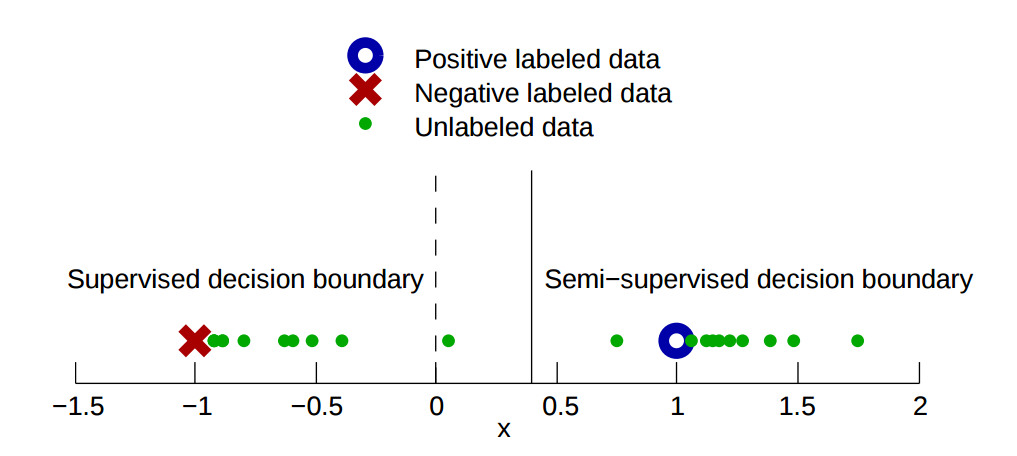
\includegraphics[width=0.95\columnwidth]{ssl.png}
  \caption{An illustrative example on how semi-supervised learning helps
    the model have a better performance.}~\label{fg:ssl_model}
\end{figure}

\subsection{Co-training}
Co-training \cite{blum1998combining} is a technique in semi-supervised learning that requires two
views of the data. It assumes that each example is described using two
different feature sets that provide different, complementary
information about the example. Co-training first learns a separate
classifier for each view using any labeled examples. The most
confident predictions of each classifier on the unlabeled data are
then used to iteratively construct additional labeled training
data. The details of co-training algorithm is described in Algorithm~\ref{algo:co-training}.
\begin{algorithm}[h] \label{algo:co-training}
  \SetKwInOut{Input}{Input}
  \Input{labeled data $\left \{ (\mathbf{x}_i, y_i)
\right \}_{i=1}^{l}$, unlabeled data $\left \{ \mathbf{x}_j
\right \}_{j=l+1}^{l+u}$ \\
each instance has two views $\mathbf{x}_i=\left [ \mathbf{x}_i^{(1)},
  \mathbf{x}_i^{(2)} \right ]$ \\
and a learning speed $k$
}
Let $L_1 = L_2 = \left \{ (\mathbf{x}_1, y_1), \ldots, (\mathbf{x}_l, y_l)
\right \}.$ \\
\Repeat {unlabeled data is used up}{
  Train view-1 $f^{(1)}$ from $L_1$, view-2 $f^{(2)}$ from $L_2$ \\
  Classify unlabeled data with $f^{(1)}$ and $f^{(2)}$ separately. \\
  Add $f^{(1)}$'s top $k$ most-confident predictions $(\mathbf{x},
  f^{(1)}(\mathbf{x}))$ to $L_2$ \\
  Add $f^{(2)}$'s top $k$ most-confident predictions $(\mathbf{x},
  f^{(2)}(\mathbf{x}))$ to $L_1$ \\
  Remove these from the unlabeled data.
}

\caption{Co-training Algorithm for Semi-Supervised Learning}
\end{algorithm}

There are three important assumptions which guarantee the performance of
co-training algorithm: 1). feature split $x=[x^{(1)};x^{(2)}]$
exists; 2). $x^{(1)}$ or $x^{(2)}$ alone is sufficient to train a good
classifier; 3). $x^{(1)}$ and $x^{(2)}$ are conditionally independent
given the class.

\subsection{Application in PeerASSIST}
Semi-supervised learning approaches come in handy in PeerASSIST when
we try to learn a function to predict the effectiveness of peer
explanations. In the setting of PeerASSIST, not every peer explanation will be received by students,
and thus, some of the explanations have no observed data on their
effectiveness (e.g., the popularity, next problem correctness). When
learning the function, these peer explanations without observed data
are discarded, which is a waste of the data. Moreover, if there are not enough
observed data, it becomes difficult to accurately learn the
function. Semi-supervised learning approaches can be applied in this
scenario to learn a better function.

\section{Natural Language Processing for Enhancing Learning}
\subsection{Confusion Detector}
Given the enormous student/instructor ratio in a MOOC's discussion
forums, it is difficulty for an instructor to read all posts in a
MOOC's discussion forums. To address this issue, \cite{Agrawal2015-hp}
collected and created the Stanford MOOCPosts dataset: a corpus
composed of 29,604 anonymized learner forum posts from eleven Stanford
University public online classes. Each post in the MOOCPosts dataset
was scored across six dimensions -- confusion, sentiment, urgency,
question, answer, and opinion -- and subsequently augmented with
additional metadata. Then the authors built a confusion classifier from
the Stanford MOOCPost dataset to automatically detect confusion from
students posts and proposed a recommendation algorithm, which takes the
student confusion as input, to automatically recommended a
video lecture from a collection of several video lectures related to
the course.
\subsection{Automated Essay Scoring}
Automated grading is a critical part of Massive Open Online Courses (MOOCs) system and any intelligent tutoring systems (ITS) at scale. Essay writing is usually a common student assessment process in schools and universities. In this task, students are required to write essays of various length, given a prompt or essay topic. Some standard tests, such as Test of English as a Foreign Language (TOEFL) and Graduate Record Examination (GRE), assess student writing skills. Manually grading these essay will be time-consuming. Thus automated essay scoring (AES) systems has been used in these tests to reduce the time and cost of grading essays. Moreover, as massive open online courses (MOOCs) become widespread and the number of students enrolled in one course increases, the need for grading and providing feedback on written assignments are ever critical.

AES has employed numerous efforts to improving its performance. AES uses statistical and Natural Language Processing (NLP) techniques to automatically predict a score for an essay based on the essay prompt and rubric. Most existing AES systems are built on the basis of predefined features, e.g. number of words, average word length, and number of spelling errors, and a machine learning algorithm \cite{Chen2013-zw}. It is normally a heavy burden to find out effective features for AES. Moreover, the performance of the AES systems is constrained by the effectiveness of the predefined features. Recently another kind of approach has emerged, employing neural network models to learn the features automatically in an end-to-end manner \cite{Taghipour2016-ns}. By this means, a direct prediction of essay scores can be achieved without performing any feature extraction. The model based on long short-term memory (LSTM) networks in \cite{Taghipour2016-ns} has demonstrated promise in accomplishing multiple types of automated grading tasks.

\subsection{NLP in PeerASSIST}
The goal of PeerASSIST is to crowdsource the explanation (in the
format of texts) of how to solve a
given problem from students and apply multi-armed bandit algorithm to
efficiently select the most helpful and useful peer explanation from all collected
peer explanations for a given problem. The effectiveness of each peer
explanations is measured in three dimensions: teacher's rating (thumb
up or thumb down), student's rating (thumb up or thumb down), and the
student next problem correctness after receiving the peer explanation.

A potential application of NLP techniques to PeerASSIST is to build a
classifier to predict the probability of a peer explanation being an
effective one based on the content of the explanation. As mentioned
above, NLP techniques, especially deep learning approaches for NLP,
have achieved promising results on text classification tasks. The
predicted probabilities can potentially used to select the optimal
explanation when one is needed to be delivered to the students. In
this scenario, we can deliver the explanation with the highest
probability to students. Another possible use of the predicted
probabilities is to treat these values as a part of the contextual
information for the explanations and incorporate this contextual
information into contextual multi-armed bandit algorithms.

The explanations collected from students are not always of good
quality. Since the classifier can automatically detect explanations
with bad quality (i.e., the explanations with low probability values),
one can quickly filter out these potential bad explanations, which
saves multi-armed bandit algorithm from wasting attempts trying these
explanations. When the explanations
that students type in are detected as bad ones by the classifier, we
can also build an intervention by
telling students that the algorithm thinks that their explanations
need some improvement. Then the students have a second chance to
submitting new explanations. We hope that there will be observable
improvement on the quality of peer explanations for these students.

\section{Reliable Crowdsourcing}
During this process of asking
students to rate the learning artifacts, we might
gather noisy rating from students due to the fact that students may
have a wide ranging level of rating expertise which are unknown, and
in some cases may be adversarial. To learn the ground truth of these
learning artifacts, we need to aggregate their opinions to recover the
true, unknown label of each learning artifacts.

\subsection{Majority Voting}
Given each item is labeled by different workers, it is a
straightforward approach to take the majority label as the true
label. From reported experimental results on real crowdcourcing data
\cite{Snow2008-rm}, majority voting performs significantly better on
average than individual workers. However, majority voting considers
each item independently and gives the same weight across all workers
who label the item when aggregating true label.

\subsection{Dawid-Skene Model}
\cite{dawid1979maximum} were among the first to consider such a
problem setup. They assume each workers are conditionally independent
given the true labels and each worker is associated with a
probabilistic confusion matrix that generates her labels. Each entry
of the matrix indicates the probability that items in one class are
labeled as another. Given the
observed responses, the true labels for each items and the confusion
matrices for each worker can be jointly estimated by a maximum
likelihood method. The optimization can be implemented by the
expectation-maximization (EM) algorithm.


\subsection{GLAD}
\cite{NIPS2009_3644} proposed a richer graphic model which includes
item difficulty and the expertise of the worker. The difficulty of
item is modeled by the parameter $1/\beta_j \in [0,\infty)$. Here $1/\beta_j = \infty$
means the image is very ambiguous and hence the most proficient worker
has a random chance of labeling it correctly. $1/\beta_j = 0$ means the item is
so easy that even the most obtuse worker will always label it correctly.

The expertise of each worker $i$ is modeled using the parameter
$\alpha_i \in (-\infty, +\infty)$. Here $\alpha = +\infty$ means the
worker always labels items correctly; $-\infty$ means the worker
always labels items incorrectly.

The labels given by worker $i$ to item $j$ are denoted as $L_{ij}$
and are generated as follows:

\begin{equation} \label{eq:glad_label}
  p(L_{ij}=Z_j|\alpha_i , \beta_j) = \frac{1}{1+e^{-\alpha_i \beta_j}}
\end{equation}

As the difficulty $1/\beta_j$ of an item increases, the probability of
the label being correct moves toward 0.5. Similarly, as the worker's
expertise decreases (lower $\alpha_i$), the chance of correctly
labeling drops to 0.5. Figure~\ref{fg:glad_model} shows the structure
of the graphical model.

\begin{figure}[h]
  \centering
  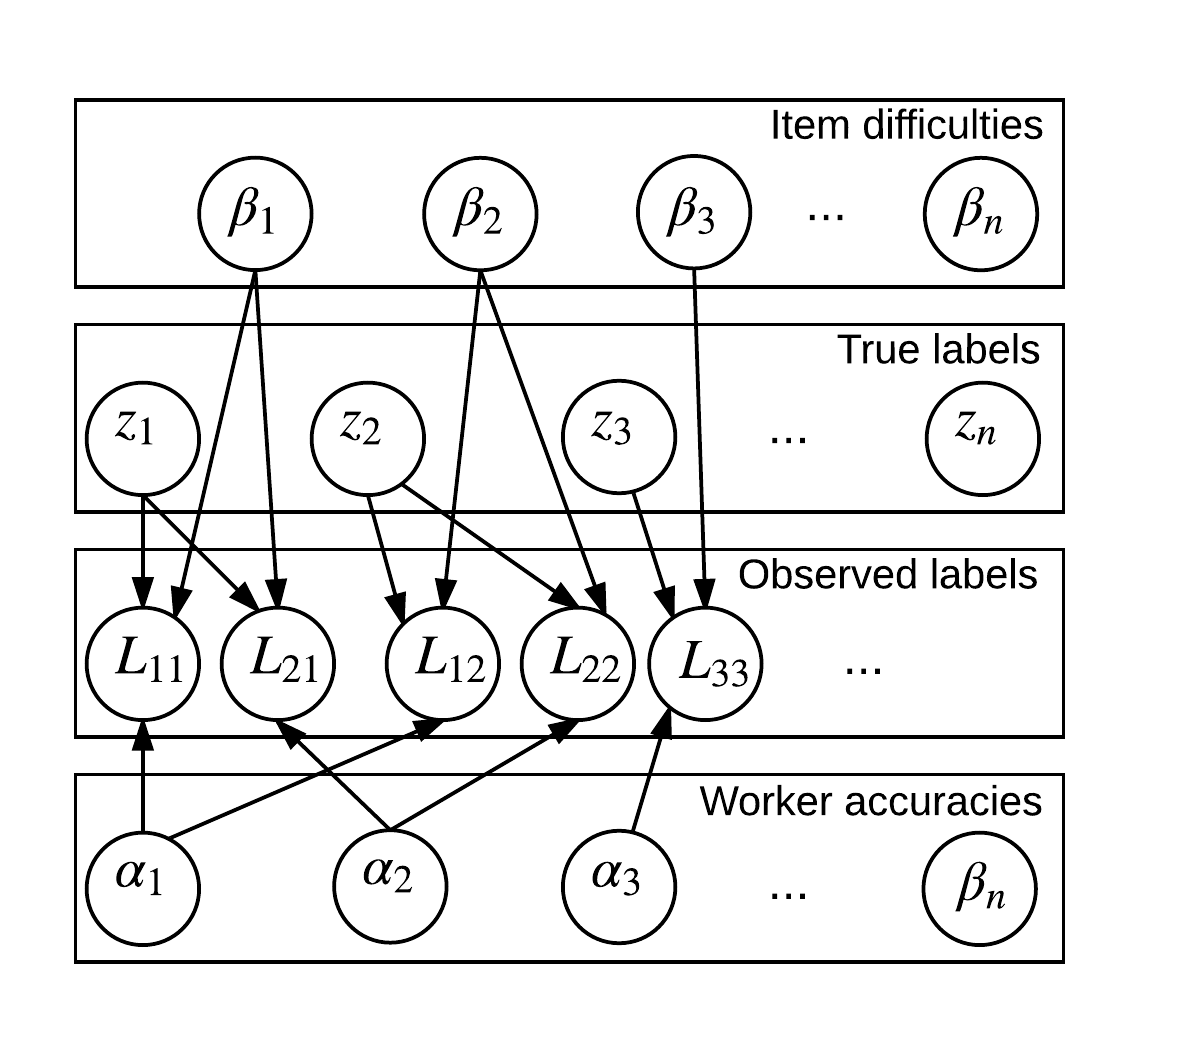
\includegraphics[width=0.95\columnwidth]{glad.png}
  \caption{An illustrative example on how semi-supervised learning helps
    the model have a better performance.}~\label{fg:glad_model}
\end{figure}

\subsection{Deep Learning Approach}
\cite{Shaham2016-nh} showed that the Dawid and Skene model is
equivalent to a Restricted Boltzmann Machine (RBM) with a single
hidden node under the assumption that all workers are conditionally
independent. Thus the posterior probabilities of the true labels can
be estimated via a trained RBM.

A RBM is an undirected bipartite graphical model, consisting of a
visible layer $X$ and a hidden layer $H$. The visible layer consists
of $d$ binary random variables and the hidden layer $m$ binary random
variables. These two layers are fully connected to each other. A RBM
is parametrized by $\lambda = (W, a, b)$, where $W$ is the weight
matrix of the connections between the visible and hidden units, and
$a,b$ are the bias vectors of the visible and hidden layers,
respectively. An illustration of a RBM is depicted in Figure~\ref{fg:rbm_model}.

A RBM implies the conditional probabilities

\begin{align*}
p_{\lambda}(X_i=1|H) &= \sigma (a_i+W_{i\cdot}H) \\
p_{\lambda}(H_j=1|X) &= \sigma (b_j+X^{T}W_{\cdot j}),
\end{align*}
where $\sigma (z)$ is the sigmoid function, $W_{i\cdot}$ is the $i$-th
row of $W$ and $W_{\cdot j}$ is its $j$-th column.
\begin{figure}[h]
  \centering
  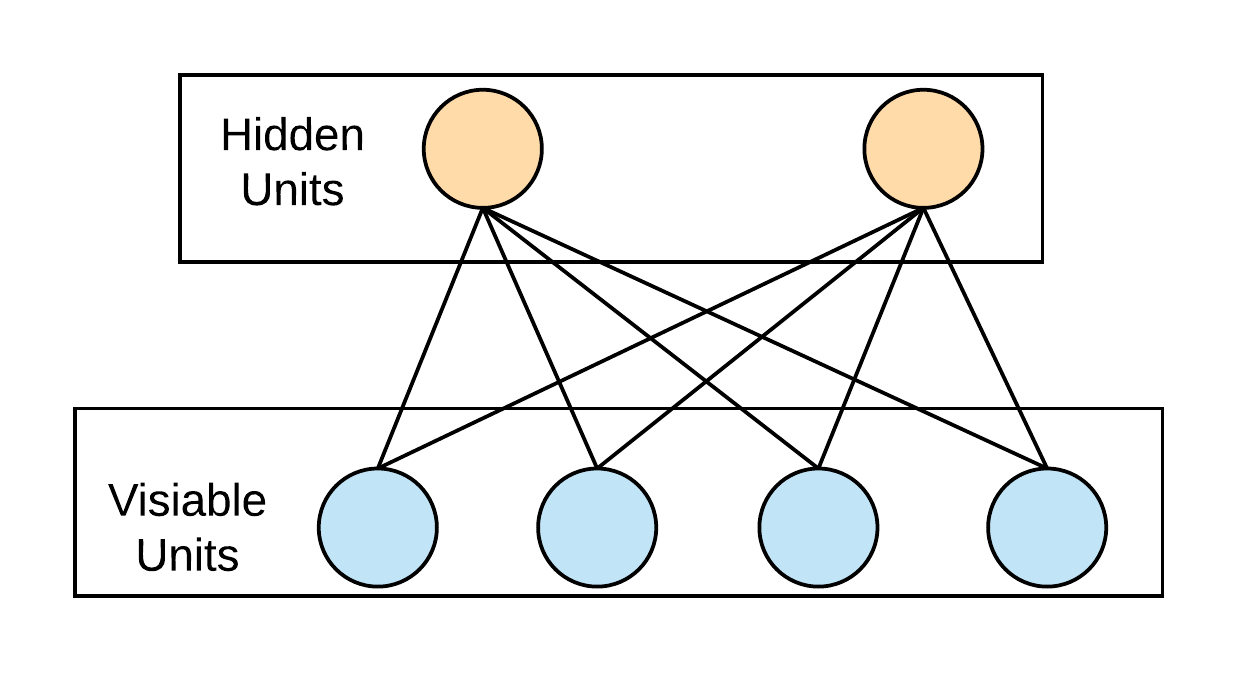
\includegraphics[width=0.95\columnwidth]{rbm.png}
  \caption{Diagram of a restricted Boltzmann machine with four visible
  units and three hidden units (no bias units)} ~\label{fg:rbm_model}
\end{figure}

To relax the assumption on the conditional independence of the
variables $X_1,\ldots,X_d$, a RBM-based Deep Neural Net (DNN) is
proposed to estimate the posterior probabilities
$p_{\theta}(Y|X)$. The mechanism to stack multiple RBMs is that the
hidden layer of each RBM is the input for the successive RBM. The RBMs
are trained one at a time from bottom to top. Specifically, given
training data $x^{(1)}, \ldots, x^{(n)} \in \{ 0,1 \}^d$, the bottom
RBM is trained first, and then obtain the hidden representation of the
first layer by sampling $h^{(i)}$ from the conditional RBM
distribution $p_{\lambda}(H|X=x^{(i)})$. The vector $h^{(1)}, \ldots,
h^{(n)}$ are then used as a training set for the second RBM and so
on. An illustration of a RBM is depicted in Figure~\ref{fg:rbm-dnn-model}.

\begin{figure}[h]
  \centering
  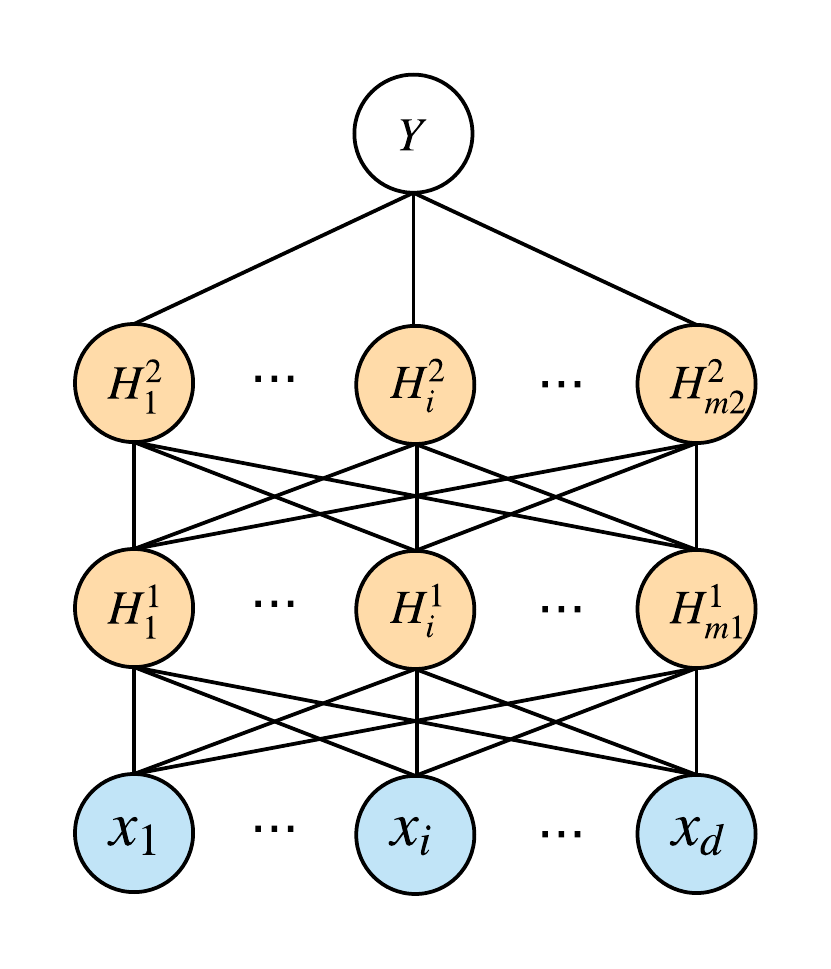
\includegraphics[width=0.75\columnwidth]{rbm-dnn.png}
  \caption{Diagram of RBM-based DNN with two hidden layers.}
  ~\label{fg:rbm-dnn-model}
\end{figure}

\subsection{Minimax Entropy}
\cite{Zhou2012-ry} proposed a minimax entropy principle to estimate
the ground truth given the observed labels by workers. The model is
illustrated in Figure~\ref{fg:minimax_entropy_model}. Each row
corresponds to a works indexed by $i$ (from 1 to $m$). Each column
corresponds to an item to be labeled, indexed by $j$ (from 1 to
$n$). Each item has an unobserved label represented as a vector
$y_{jl}$, which is 1 when item $j$ is in class $l$ (from 1 to $c$),
and 0 otherwise. Observed data is a tensor of labels $z_{ijk}$, which
is 1 when the item $i$ is labeled as class $j$ by the worker $i$, and
0 otherwise. We assume that $z_{ij}$ are drawn from
$\pi_{ij}$. $\pi_{ij}$ can be represented as a tensor $\pi_{ijk}$,
which is the probability that worker $i$ labels item $j$ as class
$k$. The proposed model will estimate $y_{jl}$ from the observed
$z_{ij}$.
\begin{figure}[h]
  \centering
  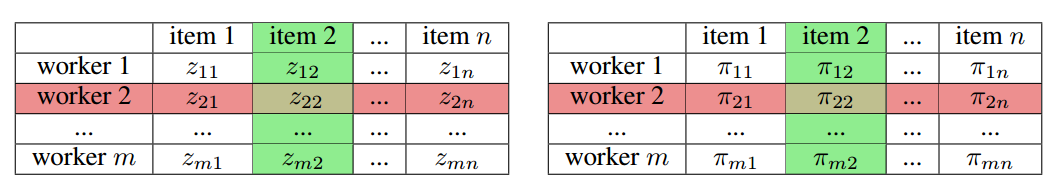
\includegraphics[width=0.95\columnwidth]{minimax_entropy.png}
  \caption{Left: observed labels. Right: underlying
    distributions. Highlights on both tables indicate that rows and
    columns of the distributions are constrained by sums over observations.}
  ~\label{fg:minimax_entropy_model}
\end{figure}

The maximum entropy model for $\pi_{ij}$ given $y_{jl}$ is as
follow:

\begin{align}
\max_{\pi} & -\sum_{i=1}^{m}\sum_{j=1}^{n}\sum_{k=1}^{c} \pi_{ijk}
\ln \pi_{ijk} \nonumber \\
  \mathrm{s.t.} & \sum_{i=1}^{m}\pi_{ijk} = \sum_{i=1}^{m}z_{ijk},
                  \forall j,k, ~ \sum_{j=1}^{n}y_{jl}\pi_{ijk} =
                  \sum_{j=1}^{n}y_{jl}z_{ijk} \forall i,k,l, \nonumber
  \\
  & \sum_{k=1}^{c}\pi_{ijk}=1, \forall i,j, \pi_{ijk} \geq 0, \forall
    i,j,k. \label{eq:max_entropy}
\end{align}

To infer $y_{jl}$, they proposed to choose $y_{jl}$ to minimize the
entropy in Equation~\ref{eq:max_entropy}.

\begin{align}
\min_{y}\max_{\pi} & -\sum_{i=1}^{m}\sum_{j=1}^{n}\sum_{k=1}^{c} \pi_{ijk}
\ln \pi_{ijk} \nonumber \\
  \mathrm{s.t.} & \sum_{i=1}^{m}\pi_{ijk} = \sum_{i=1}^{m}z_{ijk},
                  \forall j,k, ~ \sum_{j=1}^{n}y_{jl}\pi_{ijk} =
                  \sum_{j=1}^{n}y_{jl}z_{ijk} \forall i,k,l, \nonumber
  \\
  & \sum_{k=1}^{c}\pi_{ijk}=1, \forall i,j, \pi_{ijk} \geq 0, \forall
    i,j,k, \sum_{l=1}^{c}y_{jl}=1, \forall j, y_{jl} \geq 0, \forall
    j, l. \label{eq:minimax_entropy}
\end{align}

\subsection{Control Items}
Control items with known answers can be used to evaluation workers'
reliability and bias, and hence weight their answers accordingly on target
items with unknown answers. There is a trade-off in this
scenario: we can better estimate workers' reliability and bias by
letting them answer more control items, but there are fewer
opportunities left for the
target items. On the other hand, using fewer control items produces poor
estimates of worker's reliability and bias, which leads to a bad
result when aggregating workers' answers. \cite{Liu2013-ck} examined
the effectiveness of control items and provided insights on how many control items are enough under
different scenarios, which can help crowdsourcing practitioners make
their own decisions. Aforementioned methods
(except for majority voting) evaluate workers' reliability by
comparing their agreement with other workers and control items can be
incorporated into these methods.

\section{Gaussian Processes in Bandit Setting}~\label{sect:gp}
The Gaussian process is the extension of multivariate Gaussian to infinite-sized collections of real-valued variables. In particular, this extension will allow us to think of Gaussian processes as distributions not just over random vectors but in fact distributions over random functions.

The Gaussian process $\mathrm{GP}(\mu_0,k)$ is a non-parametric model
that is fully characterized by its prior mean function $\mu_0 :
\mathcal{X}\rightarrow \mathbb{R}$ and its positive-definite kernel,
or covariance function, $k: \mathcal{X} \times \mathcal{X} \rightarrow
\mathbb{R}$.

Let $\mathcal{D}_n = \left \{( \mathbf{x}_i, y_i \right )\}$ denote a
set of $n$ observations and $\mathbf{x}$ denote the arbitrary test
point. The random variable $f(\mathbf{x})$ is also a GP distribution
conditioned on observations $\mathcal{D}_n$ with following mean
$\mu_n(\mathbf{x})$ and variance $\sigma_n^2(\mathbf{x})$:
\begin{align}
 \mu_n(\mathbf{x}) &= \mu_0(\mathbf{x}) +
                     \mathbf{k}(\mathbf{x})^T(\mathbf{K}+\sigma^2\mathbf{I})^{-1}(\mathbf{y}-\mathbf{m})
  \\
  \sigma_n^2(\mathbf{x}) &= k(\mathbf{x}, \mathbf{x}) -
                           \mathbf{k}(\mathbf{x})^T(\mathbf{K}+\sigma^2\mathbf{I})^{-1}\mathbf{k}(\mathbf{x})
\end{align}
where $m_i := \mu_0(\mathbf{x}_i)$, $K_{i,j} := k(\mathbf{x_i, x_j})$,
and $\mathbf{k}(\mathbf{x})$ is a vector of covariance terms between
$\mathbf{x}$ and $\mathbf{x}_{1:n}$.

The posterior mean and variance evaluated at any point $\mathbf{x}$
represent the model's prediction and uncertainty in the objective
function at the point $\mathbf{x}$. In order to apply GP under the
setting of multi-armed bandit, we need a acquisition function to select
the next query point given the posterior model. The acquisition
function should be carefully design to trade off exploration of the
search area and exploitation of current promising areas.

\subsection{GP-UCB}
To decrease uncertainty globally, one strategy could be to pick the
point which maximums the variance $\mathbf{x}_{n+1}=
\underset{\mathbf{x} \in
  D}{\mathrm{arg\,max}}~\sigma_n(\mathbf{x})$. However, this strategy
is not well suited for multi-armed bandit problem since it can be
wasteful. Another idea is to
select the point which maximizes the expected reward given the
posterior model $\mathbf{x}_{n+1}=
\underset{\mathbf{x} \in
  D}{\mathrm{arg\,max}}~\mu_n(\mathbf{x})$. However, this idea is too
greedy and tends to end up with a local optima. To balance exploration
and exploitation, a combined strategy is to choose
\begin{equation}
  \mathbf{x}_{n+1} = \underset{\mathbf{x} \in D}{\mathrm{arg \,
      max}}\,\mu_n(\mathbf{x})+\beta_n \sigma_n(\mathbf{x}),
\end{equation} \label{eq:gp-ucb-query}
where $\beta_n$ are constants. There are theoretically motivated
guidelines for setting and scheduling the hyperparameter $\beta_n$ to
achieve optimal regret.

Since Equation~\ref{eq:gp-ucb-query} is an upper confidence bound of
the marginal posterior $P(f(\mathbf{x})|\mathbf{y}_n)$, a natural
interpretation of this strategy is that it selects the point
$\mathbf{x}$ such that $f(\mathbf{x})$ is a reasonable upper bound on
$f(\mathbf{x})$. This algorithm is called Gaussian process upper
confidence bound (GP-UCB), introduced by \cite{Srinivas2010-hi}. The
GP-UCB selection rule is motivated by the UCB algorithm for the
classical multi-armed bandit problem.

\subsection{Contextual GP-UCB}
Motivated by GP-UCB algorithm mentioned above, \cite{Krause2011-sb}
extended the generalization of this algorithm by incorporating
contextual information
\begin{equation}
  \mathbf{x}_{n+1} = \underset{\mathbf{x} \in D}{\mathrm{arg \,
      max}}\,\mu_n(\mathbf{x}, \mathbf{z}_n)+\beta_n
  \sigma_n(\mathbf{x}, \mathbf{z}_n),
\end{equation} \label{eq:cgp-ucb-query}
where $z_n \in Z$ is the contextual information from a set $Z$ of
contexts, $\mu_n(\cdot)$ and $\sigma_n^2(\cdot)$ are the posterior mean
and variance of the GP conditioned on observations $\mathcal{D}_n =
\left \{( \mathbf{x}_i, \mathbf{z}_i, y_i \right )\}.$ The authors
called the selection rule the contextual Gaussian process UCB
algorithm (GCP-UCB).

To derive the kernel $k$ on the product space $Z\times X$ of contexts and
actions, a natural approach to start with kernel functions $k_Z:
Z\times Z \rightarrow \mathbb{R}$ and $k_X:X \times X \rightarrow
\mathbb{R}$ on the space of contexts and actions. \cite{Krause2011-sb}
proposed two possibilities of constructing composite kernel $k$ from
context kernel $k_Z$ and action kernel $k_X$. One is to calculate a
product kernel $k=k_Z\otimes k_X$, by setting
\begin{equation}
  (k_Z\otimes k_X)((\mathbf{z}, \mathbf{x}),(\mathbf{z}^{\prime},
  \mathbf{x}^{\prime})) = k_Z(\mathbf{z}, \mathbf{z}^{\prime})k_X(\mathbf{x}, \mathbf{x}^{\prime}).
\end{equation}

An alternative is to calculate the additive kernel $k=k_Z\oplus k_X$,
by setting

\begin{equation}
  (k_Z\oplus k_X)((\mathbf{z}, \mathbf{x}),(\mathbf{z}^{\prime},
  \mathbf{x}^{\prime})) = k_Z(\mathbf{z}, \mathbf{z}^{\prime})+k_X(\mathbf{x}, \mathbf{x}^{\prime}).
\end{equation}

\section{Propensity Score Matching}
A propensity score \cite{rosenbaum1983central} is the probability of a unit (e.g., student,
classroom, school) being assigned to a particular treatment given a
set of observed features. Propensity scores are used to reduce
selection bias by equating groups based on these features.

Suppose that we have a binary treatment $T=\{0,1\}$, an outcome $Y$, and
observed features $X$. The propensity score is defined as the
conditional probability of treatment given background variables:
$$p(x):= \Pr(T=1 \mid X=x)$$
Let $Y(0)$ and $Y(1)$ denote the potential outcomes under the control
and the treatment, respectively.

Due to random treatment assignment in RCT, the propensity score is
known. However, the actual propensity score in observational experiments is
unknown and it can be estimated using statistical or machine
learning models from the experiment data. The most commonly used model
is a logistic regression model, in which treatment assignment $T$ is
the dependent variable and features $X$ are independent variables. Beyond logistic regression, the
use of bagging or boosting \cite{Lee2010-zr}, tree-based model
(Propensity trees) and causal random forests
\cite{wager2015estimation}, and neural networks
\cite{setoguchi2008evaluating} have been proposed to estimate the
propensity score.

The purpose of Propensity score matching (PSM) \cite{austin2011introduction} is to form matched sets
of the treated and
the control subjects who share a similar value of the predicted propensity
score. PSM allows one to estimate the average treatment effect for the
treated (ATT) \cite{imbens2004nonparametric}. The ATT is the average effect of treatment on those
subjects who ultimately receive the treatment. The most common
implementation of PSM is one-to-one or pair matching, in which pairs
of the control and the treated subjects are formed, such that matched
subjects have similar values of the propensity score. Once a matched
sample has been formed, the treatment effect can be estimated by
directly comparing outcomes between treated and untreated subjects in
the matched sample. In summary, the analysis of a propensity score matched sample can mimic that of an
RCT: one can directly compare outcomes between the treated and the control
subjects within the propensity score matched sample. 

The possibility of bias arises because the apparent difference in outcome between these two groups of units may depend on characteristics that affected whether or not a unit received a given treatment instead of due to the effect of the treatment per se. In randomized experiments, the randomization enables unbiased estimation of treatment effects; for each covariate, randomization implies that treatment-groups will be balanced on average, by the law of large numbers. Unfortunately, for observational studies, the assignment of treatments to research subjects is typically not random. Matching attempts to mimic randomization by creating a sample of units that received the treatment that is comparable on all observed covariates to a sample of units that did not receive the treatment.

\section{Peer Review}
After going through Chris Schunn's publications, I find these three papers
\cite{patchan2016understanding,kaufman2011students,patchan2015understanding}
related to my dissertation. The summary of research findings from
these paper is listed below.

\cite{patchan2016understanding} pointed out that research on such peer assessments has found that, in general, peers
are capable of providing valid ratings, and their feedback is usually
just as effective as an instructor's feedback in help students improve
their draft and sometimes more effective. Further, participating in
peer assessment improves writing ability.

\cite{kaufman2011students} found that students
sometimes regard peer assessment as unfair and often believe that peers are
unqualified to review and assess students’ work. Furthermore, students’ perceptions about
the fairness of peer assessment drop significantly following students’ experience in doing
peer assessment. Students’ fairness perceptions—and drops in those perceptions—are most
significantly associated with their perceptions about the extent to which peers’ feedback is
useful and positive. However, students’ perceptions appear to be unrelated to the extent of
their revision work.

\cite{patchan2015understanding} found that reviewer ability and text quality did not affect the amount of
feedback provided (i.e., number of comments and length of
comments). Low reviewer provided more praise than high reviewers
whereas high reviewers provided more criticism than low
reviewers. This criticism described more problems and offered more
solutions. There was one interesting interaction between reviewer
ability and text quality -- high reviewers described more problems in
the low-quality texts than in the high-quality texts, whereas low
reviewers did not make this distinction.

\cite{patchan2016understanding} found several interesting interactions
between two factors. Often lower-ability writers benefited more from
receiving feedback from lower-ability reviewers, while higher-ability
writers benefited equally from receiving feedback from lower-ability
and higher-ability reviewers.

\section{Learnersourcing Subgoal Labels}
\cite{Weir2015-hg} presented a three-stage workflow for learners to generate
subgoal labels for how-to video while they are learning from the
videos. The goal of the first stage (Generation) is to let learners submit the
subgoal labels after a certain interval during watching the
videos. The goal of the second stage (Evaluation) is to let learners select the
most relevant answer for the video section, as well as discard
potential spam answers. The goal of the third stage (Proofreading) is
to let learners evaluate the most popular subgoal labels from stage 2
for quality and eventually agree on a final label for that
subgoal. During stage 2 and stage 3, learners always have a option to
refine the label.

In PeerAssist, only students who receive 0 on a problem are
prompted with a peer explanation from one of students who answer the same
problem correctly. Then these students have a option to give a rating
(thumb up or thumb down) to the peer explanation that they
receive. The students, who answer the problem correctly in the first
attempt, do not have a chance seeing and rating the peer
explanations. If
a certain problem is relatively easy, there will be few students who
receive 0 and it is difficult to find the optimal peer explanations
based on students' ratings. Even if the problem is relatively
difficult, we miss the contribution from the students with correct
answer in the first attempt when deciding the optimal peer
explanations. Motivated by \cite{Weir2015-hg}, we can apply two-stage
workflow to collect ratings from students in terms of the quality of
the peer explanations after they submit an answer. Assume that there
are several peer explanations available for a given problem and the
ranking of these peer explanations are already decided by some
algorithm (e.g., multi-armed bandit algorithm) based on the history data.

On stage 1, students are prompted with several (i.e., 3) peer
explanations and have a option to rate these explanations after they
submit an answer. The goal of this stage is to collect students'
opinions on these explanations and use these data as one of the
indicators to determine the most effective explanation and discard
spam explanations. In terms of
which explanations should be prompted to students on this stage,
several simple approaches can be applied: random selection from all
available explanations or newly added explanations. Exploration strategy can be applied in this scenario. For the purpose of
exploration, explanations with high uncertainty are prompted with
students. This strategy can potentially reduce the uncertainty of
these explanations and help multi-armed bandit algorithm efficiently
find the optimal explanations.

On stage 2, student are prompted with the currently optimal peer explanation
from the ranking algorithm and asked to evaluate whether this peer
explanation is highly effective. The goal of this stage is to let
students to evaluate the optimal explanation for quality and analog to
the goal of exploration strategy in multi-armed bandit algorithm.

\section{HCOMP \& CSCW}
\cite{Glassman2016-yy}
Personalized support for students is a gold standard in education,
but it scales poorly with the number of students. Prior
work on learnersourcing presented an approach for learners
to engage in human computation tasks while trying to learn
a new skill. Our key insight is that students, through their
own experience struggling with a particular problem, can
become experts on the particular optimizations they implement
or bugs they resolve. These students can then generate
hints for fellow students based on their new expertise. We
present workflows that harvest and organize students’ collective
knowledge and advice for helping fellow novices through
design problems in engineering. Systems embodying each
workflow were evaluated in the context of a college-level
computer architecture class with an enrollment of more than
two hundred students each semester. We show that, given
our design choices, students can create helpful hints for their
peers that augment or even replace teachers’ personalized assistance,
when that assistance is not available.

\cite{Yim2017-zt}
Group activities that use Google Docs for simultaneous
collaborative writing and editing are increasingly common
in higher education. Although studies show that
synchronous collaboration can bring multiple benefits, such
as enhanced productivity and writing quality, little is known
about these writing practices in classrooms and their impact
on students’ writing. Using a mixed method approach, we
conducted an empirical study that explores the different
styles of synchronous collaboration in 45 Google Docs
documents produced by 82 undergraduate students, and how
students’ practices affect the specific dimensions of the final
text including quality. The results suggest that (a) out of
four styles, Divide and Conquer style tended to produce
better quality text whereas Main Writer had the lowest
quality scores, and that (b) balanced participation and
amount of peer editing led to longer texts with higher
quality scores for content, evidence, but not organization or
mechanics. Given these results, we suggest several design
features for collaborative writing systems and propose
guidelines for instructional practices.

\cite{Yoon2016-nk}
New multi-modal annotation tools hold the promise of bringing the benefits of face-to-face contact to remote, asynchronous interactions. One such system, RichReview++, incorporates new techniques to improve access to the embedded multimedia commentary and allows users to annotate with new modalities, like deictic gestures. We conducted a series of field deployments of RichReview++ to characterize how these features benefit students using them for activities in the university classroom. Our first deployment investigated the use of multi-modal annotations as a way for instructors to provide feedback on student term papers. Our second deployment used annotations to support peer discussion about assigned readings in a graduate-level course. We found that presenting voice comments as interactive waveforms seems to facilitate students' consumption of the instructor's voice comments. We also found that gestural annotations clarify voice and give annotators a quick and lightweight way to alter the scope of their voice comments. Based on these results, we suggest ways to best leverage multi-modal annotation tools in education environments.

\bibliographystyle{apalike}
\bibliography{references}
\end{document}

%%% Local Variables:
%%% mode: latex
%%% TeX-master: t
%%% End:
